\section{Motivating Case Study: What to Capture?}
\label{sec:dataset:architecture:what_to_capture}

Let us consider the motivating case study of marathon races and determine the model of our dataset. What features do we want to capture from images within our dataset? To answer this question, we need to consider what information we see as relevant in a standard marathon photo (such as \cref{fig:introduction:background:sample_rbns}). We will consider five distinct features in the following sections.

\subsection{Feature 1: Image-Level Features}

There are two features to describe components of the entire photo that we call \textit{Image-level} features:

\begin{enumerate}
  \item whether or not the photo is considered as \textbf{crowded} (\textsc{true} or \textsc{false}), and
  \item an \textit{optional} collection of \textbf{runners} in the photo, given that the photo is not crowded.
\end{enumerate}

\begin{figure}[th]
  \centering
  \begin{subfigure}[b]{0.4\textwidth}
    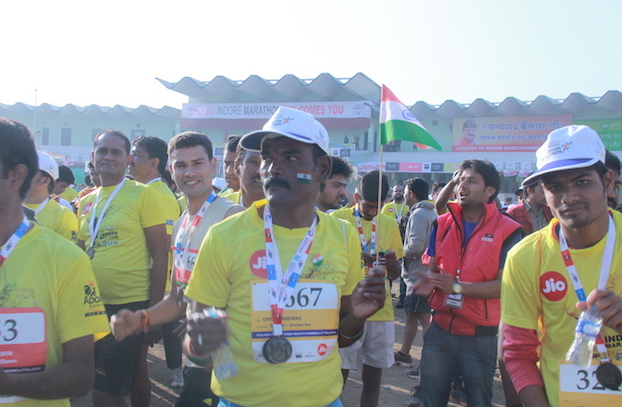
\includegraphics[width=\textwidth]{images/dataset/ImageFeatures_Crowded}
    \caption{\footnotesize A crowded photo.}
    \label{fig:dataset:image_features:crowded}
  \end{subfigure}
  \hspace{0.05\textwidth}
  \begin{subfigure}[b]{0.4\textwidth}
    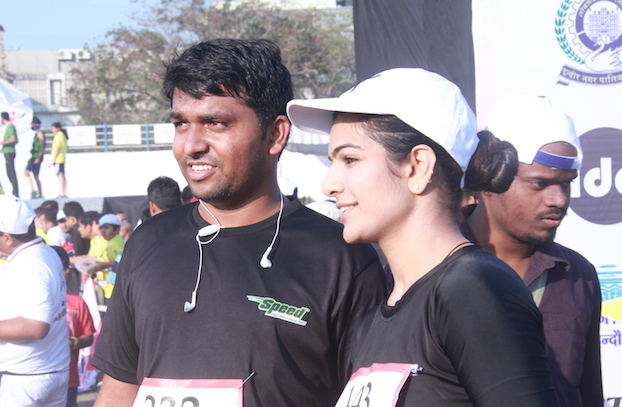
\includegraphics[width=\textwidth]{images/dataset/ImageFeatures_Optional_RBNsCropped}
    \caption{\footnotesize A photo where all \glspl{rbn} are cropped.}
    \label{fig:dataset:image_features:rbns_cropped}
  \end{subfigure}\\
  \vspace{1cm}
  \begin{subfigure}[b]{0.4\textwidth}
    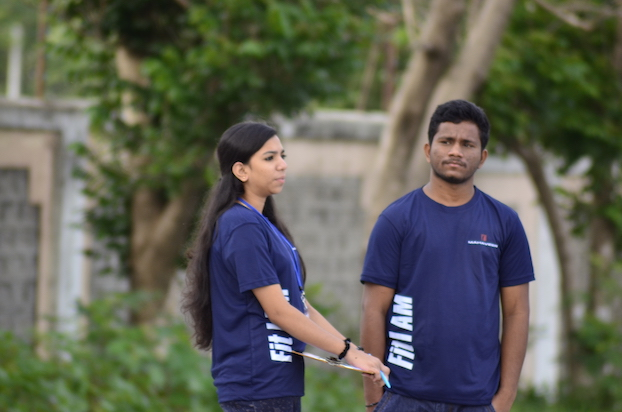
\includegraphics[width=\textwidth]{images/dataset/ImageFeatures_Optional_NoRBNs}
    \caption{\footnotesize A photo where there are no \glspl{rbn} present.}
    \label{fig:dataset:image_features:no_rbns}
  \end{subfigure} 
  \caption[Various image-level features]{Image-level features. In (a), the $PhotoCrowded$ annotation would be marked as \textsc{true}. Note the obstruction of all \glspl{rbn} in this photo. In (b) and (c), $PhotoCrowded$ is \textsc{false}, but there are no $Runners$ to tag.}
  \label{fig:dataset:image_features}
\end{figure}

We train a \gls{nn} based on photos that are not crowded; photos that are considered crowded are typically not desirable as runners prefer photos where they are the key subject. We therefore discard these photos to remove any potential bias tat the \gls{ai} could learn. We can only tag runners on the condition that the photo is not marked as crowded (\cref{fig:dataset:image_features:crowded}). Additionally, in some photos, all \glspl{rbn} are missing within the photo (e.g., hidden behind other runners, cropped out of view) and some photos contain no runners at all (\cref{fig:dataset:image_features:rbns_cropped,fig:dataset:image_features:no_rbns}). We therefore identify this as an \textit{optional} collection as we must associate an \gls{rbn} to a runner---the photo is not crowded, but there are no runners to tag, thereby making the annotation optional. Thus, an \textit{derived attribute} exists with such a collection: the \textit{count} of the runners in a photo is something we can automatically count.

\subsection{Feature 2: Bibs}

We identify the following two annotations of what we would label for a given runner's bib sheet. This is summarised in \cref{fig:dataset:bib_sheet_features}. Within this feature we identify the following annotations for \glspl{rbn}:

\begin{enumerate}
  \item a polygon around the runner's \textbf{bib sheet} that contains the $x$ and $y$ coordinates, given that there are exactly four vertices of this polygon
  \item a string with the runner's \textbf{\gls{rbn}}, once the bib sheet is tagged (exists).
\end{enumerate}

\begin{figure}[p]
  \centering
  \hspace{\fill}
  \begin{subfigure}[b]{0.25\textwidth}
    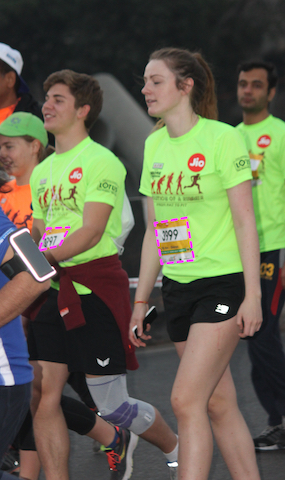
\includegraphics[width=\textwidth]{images/dataset/BibSheet_Detection}
  \end{subfigure}
  \hspace{\fill}
  \begin{subfigure}[b]{0.25\textwidth}
    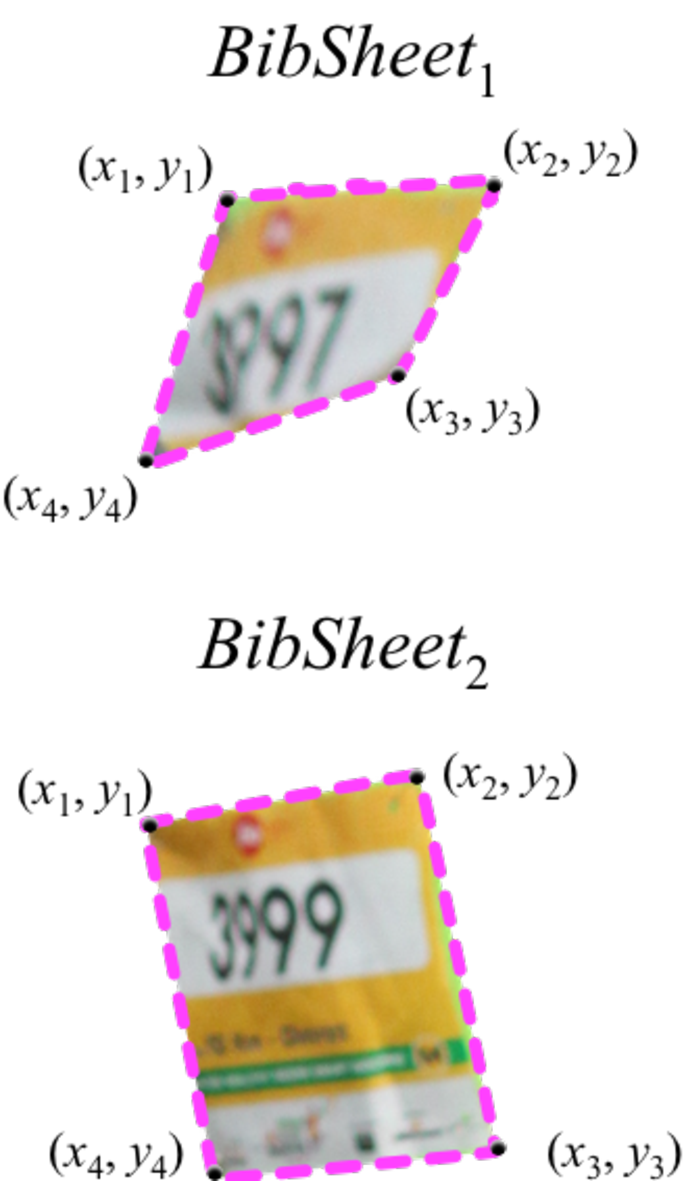
\includegraphics[width=\textwidth]{images/dataset/BibSheet_Area}
  \end{subfigure}
  \begin{subfigure}[b]{0.25\textwidth}
    
\includegraphics[width=\textwidth]{images/dataset/BibSheet_RBN}
  \end{subfigure} 
  \hspace{\fill}
  \caption[Bib Sheet segment-level features]{The bib segment-level feature. \textit{From left to right}: The manually annotated bib sheets in the original photo (outlined in magenta); the relative $BibSheet$ annotations with the four respective vertices; the detected $RBN$ input strings for the corresponding $BibSheet$.}
  \label{fig:dataset:bib_sheet_features}
\end{figure}

\subsection{Feature 3: Faces}

A further feature that is important is the runner's face region (\cref{fig:dataset:face_features}), which could compromise of five annotations:

\begin{enumerate}
  \item a rectangle around the runner's \textbf{face} that contains the two $x$ and $y$ coordinates of the two opposite vertices, given that the $bottom$ of this rectangle are above the $top$ of the bib sheet,
\end{enumerate}

\noindent
and once this face bounds has been tagged, more annotations can be extracted:

\begin{enumerate}
  \setcounter{enumi}{1}
  \item whether or not the runner is \textbf{wearing} a \textbf{hat} (\textsc{true} or \textsc{false}),
  \item whether or not the runner is \textbf{wearing} \textbf{(sun)glasses} (\textsc{true} or \textsc{false}), and
  \item the \textbf{gender} of the runner (\textsc{male}, \textsc{female}, or \textsc{unsure}).
\end{enumerate}

The bib sheet polygon would contain four \textit{explicit attributes} required as input by the tagger: the coordinates of its four vertices, $\{ (x_{1}, y_{1}), (x_{2}, y_{2}), (x_{3}, y_{3}), (x_{4}, y_{4}) \}$. Similarly, there are two explicit attributes required for the runner's face rectangle: the coordinates of the top left and the bottom right of the rectangle (i.e., the two opposite vertices) of the runner's face bounds, $\{ (x_{1}, y_{1}), (x_{2}, y_{2}) \}$. As both of these are shapes, we can automatically calculate the derived attributes from these coordinates:  $\{ top, left, bottom, right, width, height \}$.

\begin{figure}[p]
  \centering
  \hspace{\fill}
  \begin{subfigure}[b]{0.25\textwidth}
    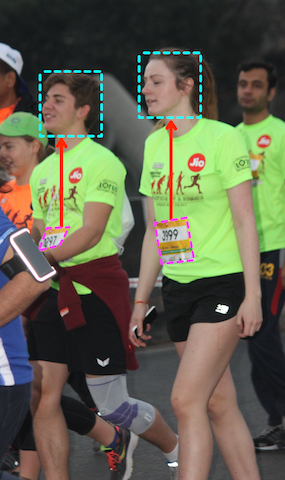
\includegraphics[width=\textwidth]{images/dataset/FaceBounds_Detection}
  \end{subfigure}
  \hspace{\fill}
  \begin{subfigure}[b]{0.25\textwidth}
    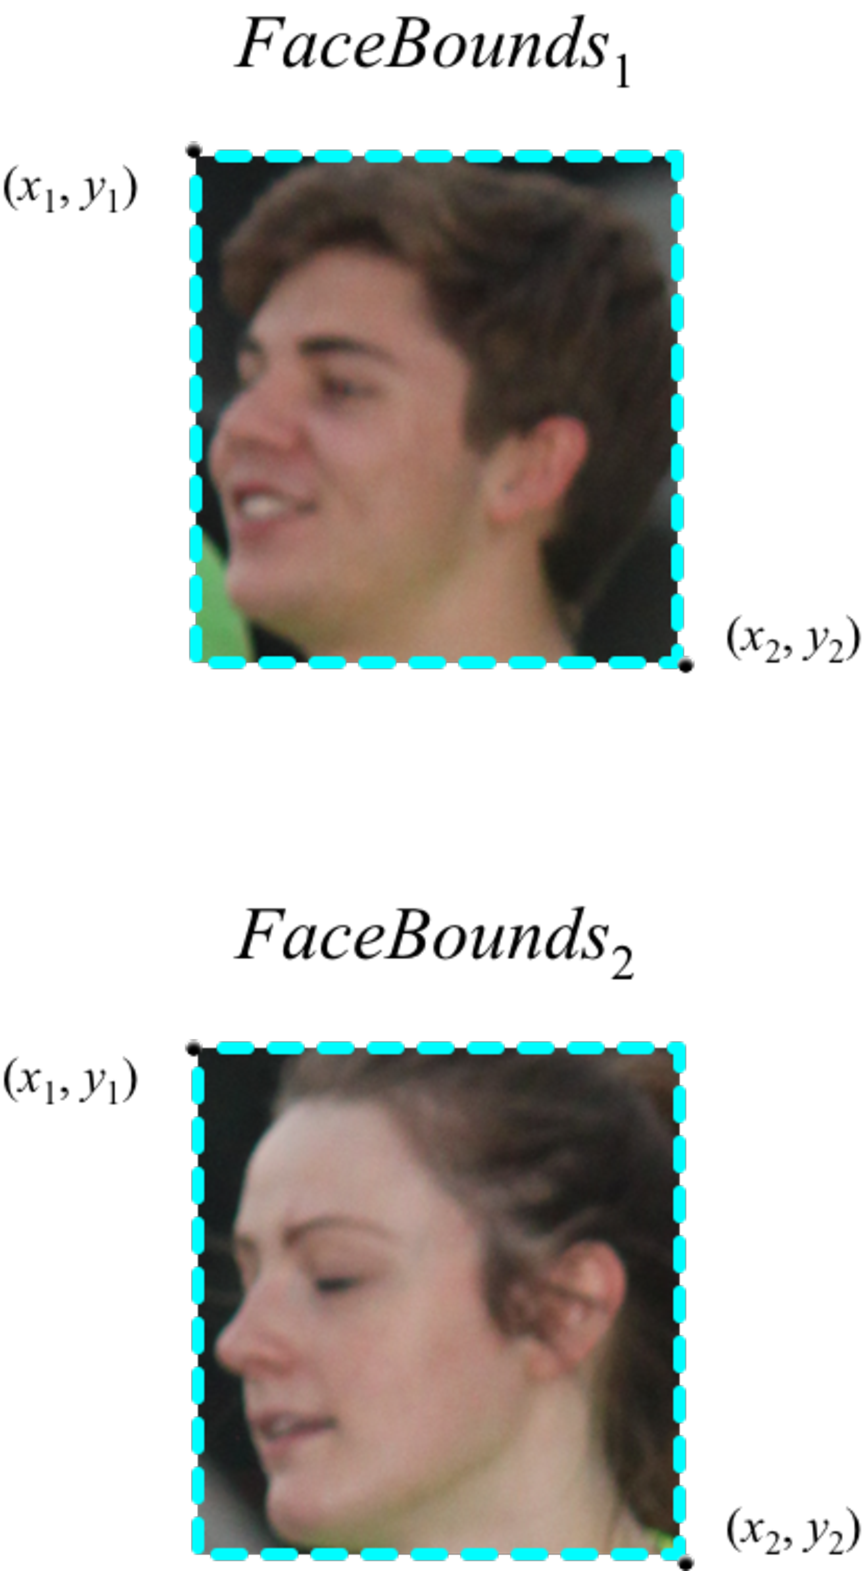
\includegraphics[width=\textwidth]{images/dataset/FaceBounds_Area}
  \end{subfigure}
  \hspace{\fill}
  \caption[Face Bounds segment-level features]{The face segment-level feature. \textit{Left}: The manually tagged face regions (cyan) that comply with the conditions that the bottom must be above the top of the bib (red arrows). \textit{Right}: the relative $FaceBounds$ annotations with the two opposite vertices. Other annotations in this feature would be: $WearingHat{1,2} = WearingGlasses{1,2} = \textsc{false}$, $Gender_{1} = \textsc{male}$, $Gender_{2} = \textsc{female}$.}
  \label{fig:dataset:face_features}
\end{figure}

%Given that the face region is tagged, we can then annotate:
%
%\begin{enumerate}
%  \item the `base classifications' of the person, and
%  \item the `colour classifications' of the person.
%\end{enumerate}

\subsection{Feature 4: Prominence}

We can now identify another feature, the prominence of the runner within the photo. These would consist of three annotations:

\begin{enumerate}
  \item whether or not the runner's \textbf{face} is \textbf{visible} (\textsc{true} or \textsc{false}),
  \item whether or not the runner is \textbf{blurry} (\textsc{true} or \textsc{false}),
  \item the \textbf{\gls{lop}} that the runner buys the photo (\textsc{no}, \textsc{maybe}, \textsc{yes}),
\end{enumerate}

A runner's face is considered `invisible' if it is obstructed by another object, cropped out of the image, or if the runner is looking down. See \cref{fig:dataset:face_prominence}. Runners are more likely purchase a photo if they are looking at the camera, and likewise if they are blurry in the image; these therefore have a significant impact on their prominence. We also define the \glsx{lop} value as a qualitative metric. We ask the data tagger to `picture' themselves as runner, and if so, we ask if they would purchase it. We then use this metric to train positive samples of good photos (\gls{lop} = \textsc{yes}) and samples of bad photos (\gls{lop} = \textsc{no}). Where \textsc{maybe} is provided, the runner is ignored to prevent training the network with indeterminate samples. Refer to \cref{fig:dataset:lop_prominence} for examples of the varying \gls{lop} values. 

\begin{figure}[p]
  \centering
  \hspace{\fill}
  \begin{subfigure}[b]{0.25\textwidth}
    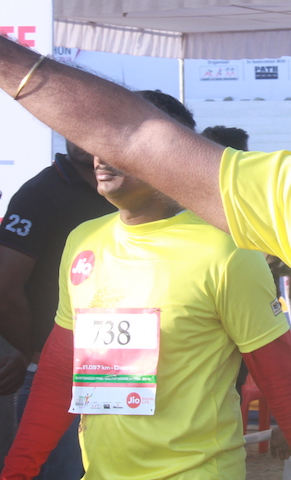
\includegraphics[width=\textwidth]{images/dataset/Prominence_FaceNotVisible_Covered}
    \caption{Face obstructed}
  \end{subfigure}
  \hspace{\fill}
  \begin{subfigure}[b]{0.25\textwidth}
    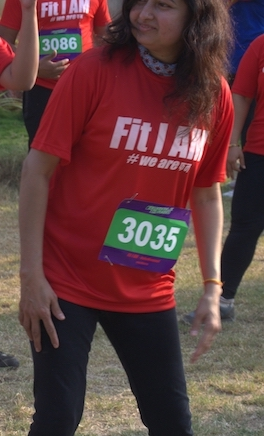
\includegraphics[width=\textwidth]{images/dataset/Prominence_FaceNotVisible_Cropped}
      \caption{Face cropped}
  \end{subfigure}
  \hspace{\fill}
  \begin{subfigure}[b]{0.25\textwidth}
    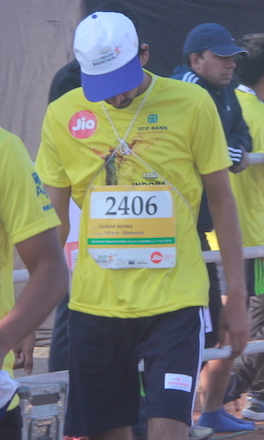
\includegraphics[width=\textwidth]{images/dataset/Prominence_FaceNotVisible_LookingDown}
    \caption{Face looking down}
  \end{subfigure}
  \hspace{\fill}
  \caption[Face visibility and its effect on prominence]{The $FaceVisible$ plays a significant impact on the prominence feature. Above are cases where the face would be marked as not visible.}
  \label{fig:dataset:face_prominence}
\end{figure}

\begin{figure}[p]
  \centering
  \hspace{\fill}
  \begin{subfigure}[b]{0.25\textwidth}
    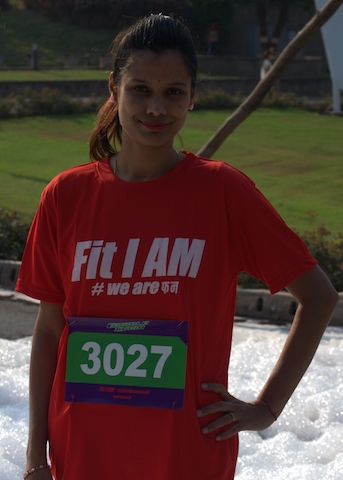
\includegraphics[width=\textwidth]{images/dataset/Prominence_LoP_Yes}
    \caption{\gls{lop} = \textsc{yes}}
  \end{subfigure}
  \hspace{\fill}
  \begin{subfigure}[b]{0.25\textwidth}
    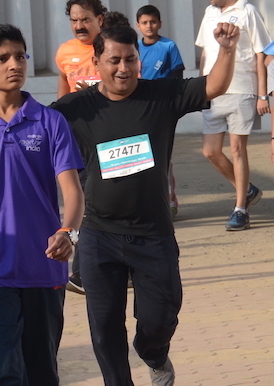
\includegraphics[width=\textwidth]{images/dataset/Prominence_LoP_Maybe}
    \caption{\gls{lop} = \textsc{maybe}}
  \end{subfigure}
  \hspace{\fill}
  \begin{subfigure}[b]{0.25\textwidth}
    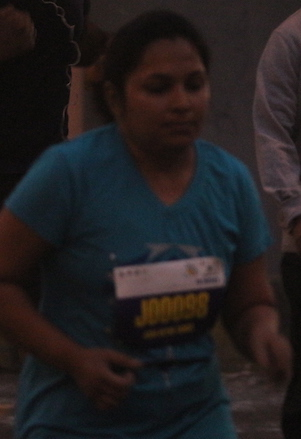
\includegraphics[width=\textwidth]{images/dataset/Prominence_LoP_No}
    \caption{\gls{lop} = \textsc{no}}
  \end{subfigure}
  \hspace{\fill}
  \caption[Variant Purchase Likelihoods]{Various examples of the $\gls{lop}$ values. In (a), the woman is clearly posing and is the primary subject of the photo. In (b), the runner is in focus in a pose, but is behind another runner and there are other runners behind him. In (c), the woman is out of focus, is blurry, and this photo has very poor lighting conditions.}
  \label{fig:dataset:lop_prominence}
\end{figure}

\subsection{Feature 5: Colours}

Another feature we can capture is a way to identify runners by the colour of their clothing. (Within our dataset, various clothing items of distinct colours are given to runners for particular races.) These features comprise of four annotations:

\begin{enumerate}
  \item an \textit{optional} \textbf{colour} of the runner's \textbf{hat}, given that they were annotated as wearing a hat,
  \item the \textbf{colour} of the runner's \textbf{shirt},
  \item an \textit{optional} \textbf{colour} of the runner's \textbf{shorts}, and
  \item an \textit{optional} \textbf{colour} of the runner's \textbf{shoes}.
\end{enumerate}

% TODO: Example of colour matching. Do we capture the coordinates?

The colour of a runner's shirt is required, as we expect that a bib would be detected on the shirt of a runner (which would be tagged). The other colour annotations are all optional, as it is likely that some of these clothing items may be cropped out of the photo or is not visible. Furthermore, the hat colour can only be specified on the condition that the tagger has marked the runner has wearing a hat.

We can segment groups of the annotations we extract into features of two categories: annotations that feature at the \textit{image}-level and those that do not, which we call \textit{segment}-level features. The image-level features are those which apply to the entire image (i.e., $PhotoCrowded$, $Runners$). Those that apply at the segment level can be grouped into what types of features we are extracting: the runner's bib, face, their prominence and their colour identification.

In summary, we have identified a total of 5 features of 15 annotations, which are summarised within \cref{tab:dataset:annotation_summary}. Each of these annotations can be classified with a name and type, conditions for the annotation to be valid, dependencies on other annotations to exist before the annotation can be made, explicit attributes which the tagger must specify, derived attributes which we can automatically compute, possible values which limit the range of data for that annotation, and whether or not the annotation is optional.

\begin{landscape}

\begin{table}[p]
  \centering
  \caption[Summary of annotations captured in the dataset]{\centering A summary of the annotations we wish to capture from our dataset. Image and segment-level features are separated using the double line.}
  \label{tab:dataset:annotation_summary}
  \tablefitlandscape{
    \begin{tabular}{llllllllll}
      \toprule
        \textbf{Feature} &
        \textbf{Annotation} &
        \textbf{Type} &
        \textbf{Conditions} &
        \textbf{Dependencies} &
        \textbf{Explicit Attributes} &
        \textbf{Derived Attributes} &
        \textbf{Possible Values} &
        \textbf{Default} &
        \textbf{Optional}
      \\
      \midrule
        \multirow{2}{*}{Image-Level} &
        $PhotoCrowded$ &
        Boolean &
        N/A &
        N/A &
        N/A &
        N/A &
        $\{ \textsc{true}, \textsc{false} \}$&
        \textsc{false} &
        No
      \\
        &
        $Runners$ &
        Collection &
        $\{ PhotoCrowded = \textsc{false} \}$ &
        N/A &
        N/A &
        $\{count\}$ &
        N/A &
        \textsc{null} &
        Yes
      \\
      \midrule
      \midrule
        \multirow{2}{*}{Bib} &
        $BibSheet$ &
        Polygon &
        $\{ vertices = 4 \}$ &
        N/A &
        $\{ x_{1} \dots x_{4}, y_{1} \dots y_{4} \}$ &
        $\{ top, left, bottom, right, width, height \}$ &
        N/A &
        \textsc{null} &
        No
      \\
        &
        $\gls{rbn}$ &
        Label &
        N/A &
        $BibSheet$ &
        N/A &
        N/A &
        N/A &
        \textsc{null} &
        No
      \\
      \midrule
        \multirow{2}{*}{Face} &
        $FaceBounds$ &
        Rectangle &
        $\{ bottom > BibSheet_{top} \}$  &
        $BibSheet$ &
        $\{ x_{1}, y_{1}, x_{2}, y_{2}\}$ &
        $\{ top, left, bottom, right, width, height \}$ &
        N/A &
        \textsc{null} &
        No
      \\
        &
        $WearingHat$ &
        Boolean &
        N/A &
        $FaceBounds$ &
        N/A &
        N/A &
        $\{ \textsc{true}, \textsc{false} \}$&
        \textsc{false} &
        No
      \\
        &
        $WearingGlasses$ &
        Boolean &
        N/A &
        $FaceBounds$ &
        N/A &
        N/A &
        $\{ \textsc{true}, \textsc{false} \}$&
        \textsc{false} &
        No
      \\
        &
        $Gender$ &
        Category &
        N/A &
        $FaceBounds$ &
        N/A &
        N/A &
        $\{ \textsc{male}, \textsc{female}, \textsc{unsure} \} $ &
        \textsc{male} &
        No
      \\
      \midrule
        \multirow{2}{*}{Prominence} &
        $\gls{lop}$ &
        Category &
        N/A &
        $FaceBounds$ &
        N/A &
        N/A &
        $\{ \textsc{no}, \textsc{maybe}, \textsc{yes} \}$ &
        \textsc{maybe} &
        No
      \\
        &
        $FaceVisible$ &
        Boolean &
        N/A &
        $FaceBounds$ &
        N/A &
        N/A &
        $\{ \textsc{true}, \textsc{false} \}$&
        \textsc{true} &
        No
      \\
        &
        $Blurry$ &
        Boolean &
        N/A &
        $FaceBounds$ &
        N/A &
        N/A &
        $\{ \textsc{true}, \textsc{false} \}$&
        \textsc{false} &
        No
      \\
      \midrule
        \multirow{2}{*}{Colours} &
        $ShirtColor$ &
        Color &
        N/A &
        $FaceBounds$ &
        $\{ red, green, blue \}$ &
        N/A &
        N/A &
        \textsc{null} &
        No
      \\
        &
        $ShoeColor$ &
        Color &
        N/A &
        $FaceBounds$ &
        $\{ red, green, blue \}$ &
        N/A &
        N/A &
        \textsc{null} &
        Yes
      \\
        &
        $ShortsColor$ &
        Color &
        N/A &
        $FaceBounds$ &
        $\{ red, green, blue \}$ &
        N/A &
        N/A &
        \textsc{null} &
        Yes
      \\
        &
        $HatColor$ &
        Color &
        $\{ WearingHat = \textsc{true} \}$ &
        $FaceBounds$ &
        $\{ red, green, blue \}$ &
        N/A &
        N/A &
        \textsc{null} &
        Yes
      \\
      \bottomrule
    \end{tabular}
  }
\end{table}

\end{landscape}

% Run through an example of what it is we need to capture for our study & why (Refer to meeting 1 notes).
% state diagram of things we need to classify (break down diagram).
